% =====================================================================
%  Container Doctor: a local LLM agent that diagnoses broken Docker containers
%  Short technical report (build: pdflatex container_doctor_report.tex, twice)
%  Ashmik Ajay Harinkhede, 2025H1030037H, BITS Pilani, Hyderabad Campus
%  Results tables are generated by make_tables.py from ../results/*.json
% =====================================================================
\documentclass[10pt,a4paper]{article}

\usepackage[T1]{fontenc}
\usepackage[utf8]{inputenc}
\usepackage{mathpazo}
\renewcommand{\ttdefault}{lmtt}
\usepackage{microtype}
\usepackage[margin=0.85in,top=0.8in,bottom=0.85in]{geometry}
\usepackage{booktabs}
\usepackage{graphicx}
\usepackage{xcolor}
\usepackage{fancyhdr}
\usepackage{lastpage}
\usepackage{caption}
\usepackage{enumitem}
\usepackage{pifont}
\usepackage{float}
\usepackage{tikz}
\usetikzlibrary{arrows.meta,positioning,fit,backgrounds}
\usepackage[hidelinks]{hyperref}

\definecolor{navy}{RGB}{0,0,128}
\definecolor{boxbg}{RGB}{240,243,250}
\hypersetup{colorlinks=true,linkcolor=navy,urlcolor=navy}
\captionsetup{font=small,labelfont=bf,skip=4pt}
\setlist{itemsep=1pt,topsep=3pt,parsep=0pt,leftmargin=14pt}
\newcommand{\cmark}{\textcolor{green!45!black}{\ding{51}}}
\newcommand{\xmark}{\textcolor{red!70!black}{\ding{55}}}
\newcommand{\code}[1]{\texttt{#1}}

\pagestyle{fancy}
\fancyhf{}
\fancyhead[L]{\small Container Doctor}
\fancyhead[R]{\small November 2026}
\fancyfoot[C]{\small Page \thepage\ of \pageref{LastPage}}
\renewcommand{\headrulewidth}{0.4pt}
\setlength{\headheight}{13pt}

\usepackage{titlesec}
\titleformat{\section}{\large\bfseries\color{navy}}{\thesection}{0.6em}{}
\titlespacing*{\section}{0pt}{8pt}{3pt}
\titleformat{\subsection}{\normalsize\bfseries}{\thesubsection}{0.5em}{}
\titlespacing*{\subsection}{0pt}{5pt}{2pt}

% Generated by report/make_tables.py from results/*.json. Do not edit.
\newcommand{\SummaryTable}{%
\begin{tabular}{llccccc}
\toprule
Mode & Run & Correct & Avg steps & Avg tool calls & Avg time (s) & Searched runbooks \\
\midrule
no\_rag & v1 & 9/15 & 4.1 & 2.4 & 36 & 0/15 \\
no\_rag & v2 & 8/15 & 4.3 & 2.5 & 38 & 0/15 \\
\midrule
rag & v1 & 12/15 & 7.7 & 4.7 & 131 & 13/15 \\
rag & v2 & 12/15 & 7.9 & 5.0 & 126 & 15/15 \\
\bottomrule
\end{tabular}}
\newcommand{\PerScenarioTable}{%
\begin{tabular}{lcccc}
\toprule
Scenario & \multicolumn{2}{c}{no\_rag} & \multicolumn{2}{c}{rag} \\
\cmidrule(lr){2-3}\cmidrule(lr){4-5}
 & v1 & v2 & v1 & v2 \\
\midrule
01 missing env var & \cmark & \cmark & \cmark & \cmark \\
02 oom killed & \cmark & \xmark & \cmark & \cmark \\
03 port conflict & \xmark & \xmark & \cmark & \cmark \\
04 db not ready & \xmark & \xmark & \cmark & \cmark \\
05 wrong volume path & \xmark & \xmark & \cmark & \cmark \\
06 permission denied & \cmark & \cmark & \cmark & \xmark \\
07 dns wrong host & \xmark & \xmark & \cmark & \cmark \\
08 crash loop & \cmark & \cmark & \cmark & \cmark \\
09 healthcheck failing & \xmark & \xmark & \xmark & \xmark \\
10 wrong command & \cmark & \cmark & \cmark & \cmark \\
11 nginx config error & \cmark & \cmark & \xmark & \cmark \\
12 binds localhost & \xmark & \xmark & \cmark & \cmark \\
13 wrong db password & \cmark & \cmark & \xmark & \cmark \\
14 disk full & \cmark & \cmark & \cmark & \xmark \\
15 missing module & \cmark & \cmark & \cmark & \cmark \\
\bottomrule
\end{tabular}}


\begin{document}

% ---------------------------------------------------------------- header
\begin{minipage}[c]{0.14\textwidth}

\includegraphics[width=\textwidth]{bits_logo.png}
\end{minipage}\hfill
\begin{minipage}[c]{0.83\textwidth}
{\LARGE\bfseries Container Doctor\par}
\vspace{2pt}
{\large A local LLM agent that diagnoses broken Docker containers\par}
\vspace{4pt}
{\small Ashmik Ajay Harinkhede \,·\, ID 2025H1030037H \,·\, M.E.\ Computer Science, BITS Pilani Hyderabad\\
Independent personal project \,·\, November 2026 \,·\,
\href{https://github.com/ashmik2005/container-doctor}{github.com/ashmik2005/container-doctor}\par}
\end{minipage}

\vspace{6pt}
\noindent\colorbox{boxbg}{\parbox{\dimexpr\textwidth-2\fboxsep}{\small
\textbf{Summary.} Container Doctor takes a plain-language complaint (``my web app is down''),
investigates the Docker host by itself through a set of read-only tools, and replies with a
root cause, the evidence for it and a fix. It runs fully offline on a laptop CPU with a
3-billion-parameter model (\code{qwen2.5:3b} via Ollama), and the tool-calling loop is written
by hand in about 250 lines of Python without any agent framework. A runbook knowledge base
(21 notes in ChromaDB) is exposed as a search tool, so the agent decides when to retrieve.
On 15 deliberately broken docker compose scenarios, the agent found the right root cause in
\textbf{12/15} cases with the runbook tool and \textbf{8/15} without it, at about 3.3$\times$ the time per
diagnosis (headline run v2, keyword scoring).}}

% ---------------------------------------------------------------- 1
\section{Problem and approach}
When a container fails, the cause is usually visible in one of a handful of places: the
container status and exit code, the last lines of its logs, its configuration in
\code{docker inspect}, or the state of a host port. Finding it means knowing \emph{where} to
look for \emph{which} symptom. This is a natural fit for a tool-using agent: the right next step
depends on what the previous step showed, so a fixed script cannot cover every case.

The project had three constraints: everything local and free (no API keys, logs never leave the
machine), no agent framework (LangChain etc.), so that every step of the loop is explicit, and
CPU-only inference on an Intel laptop. The last constraint forced a small model, and much of the
engineering was about making a small model behave reliably.

% ---------------------------------------------------------------- 2
\section{System design}

\begin{figure}[h]
\centering
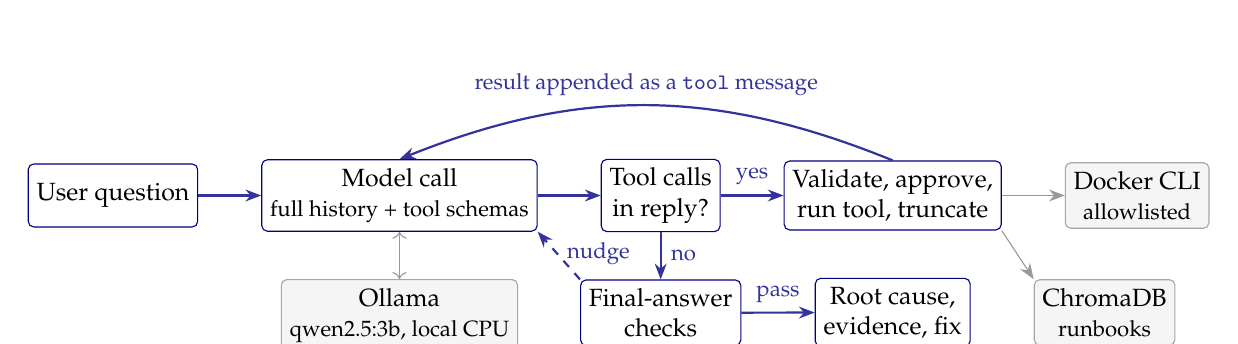
\begin{tikzpicture}[
  font=\small, node distance=6mm and 8mm,
  box/.style={draw=navy, rounded corners=2pt, fill=white, align=center, inner sep=3pt, minimum height=8mm},
  store/.style={draw=gray!70, fill=gray!8, rounded corners=2pt, align=center, inner sep=3pt, minimum height=8mm},
  arr/.style={-{Stealth[length=2mm]}, thick, navy!80},
  ext/.style={-{Stealth[length=2mm]}, gray!80}]
  % row 1: the main path
  \node[box] (user) {User question};
  \node[box, right=of user] (model) {Model call\\{\footnotesize full history + tool schemas}};
  \node[box, right=of model] (check) {Tool calls\\in reply?};
  \node[box, right=of check] (exec) {Validate, approve,\\run tool, truncate};
  % row 2
  \node[store, below=of model] (ollama) {Ollama\\{\footnotesize qwen2.5:3b, local CPU}};
  \node[box, below=of check] (guard) {Final-answer\\checks};
  \node[box, below=of exec] (ans) {Root cause,\\evidence, fix};
  % external stores
  \node[store, right=of exec] (docker) {Docker CLI\\{\footnotesize allowlisted}};
  \node[store, right=of ans] (chroma) {ChromaDB\\{\footnotesize runbooks}};
  % main loop
  \draw[arr] (user) -- (model);
  \draw[arr] (model) -- (check);
  \draw[arr] (check) -- node[above, font=\footnotesize]{yes} (exec);
  \draw[arr] (exec.north) to[bend right=22] node[above, font=\footnotesize]{result appended as a \texttt{tool} message} (model.north);
  \draw[arr] (check) -- node[right, font=\footnotesize]{no} (guard);
  \draw[arr] (guard) -- node[above, font=\footnotesize]{pass} (ans);
  \draw[arr, dashed] (guard.north west) -- node[right, font=\footnotesize, pos=0.55]{nudge} (model.south east);
  % external calls
  \draw[ext, <->] (model) -- (ollama);
  \draw[ext] (exec) -- (docker);
  \draw[ext] (exec.south east) -- (chroma.north west);
\end{tikzpicture}
\caption{The agent loop (\texttt{agent.py}). The model only proposes tool calls; the loop validates and executes
them, appends the result as a \code{tool} message and calls the model again with the whole
history. A reply without tool calls is a candidate final answer and must pass the checks; each failed check sends one corrective nudge.}
\end{figure}

\vspace{-4pt}
\subsection{The agent loop}
Tool calling is a convention between the program and the model. The request carries JSON schemas
for each tool. Qwen2.5 was fine-tuned to answer such prompts with a structured call, which Ollama
parses into a \code{tool\_calls} field, e.g.\ \code{get\_logs(container="web")}. The loop looks
the name up in a dictionary of Python functions, runs it, appends the output as a message with role
\code{tool}, and calls the model again. The model is stateless: the message list \emph{is} the
agent's memory and is resent on every step. That is why output size and step count must be bounded.

\subsection{Tools and safety}
Six tools wrap the Docker CLI and the host: \code{list\_containers}, \code{get\_logs},
\code{inspect\_container} (a 37-line summary of the 238-line \code{docker inspect} JSON),
\code{check\_port} (who publishes a port, is anything listening, what a TCP/HTTP probe returns),
\code{check\_disk} and \code{restart\_container}. A seventh, \code{search\_runbooks}, does
retrieval. Because the agent runs real commands, safety is layered:
\begin{itemize}
\item \textbf{Fixed commands, validated arguments.} The model fills in arguments only. Unknown tools
  and missing arguments become error messages it can react to; container names must match Docker's
  naming rule, which also blocks option injection such as \code{--follow}.
\item \textbf{Allowlist and no shell.} One function runs every command, only if its prefix is on a
  read-only allowlist, always with \code{subprocess.run([...])} and never \code{shell=True}.
\item \textbf{Human approval.} State-changing tools ask y/n on the terminal; with no terminal (or in
  evaluation) they are denied. Failing safe mattered in practice: the model did request restarts.
\item \textbf{Bounds.} At most 8 model calls per run, 1024 generated tokens per call, 3000 characters
  per tool result (keeping the tail, where errors are), 30\,s per command, explicit 8k context.
\end{itemize}

\subsection{Making a 3B model reliable}
The small model often ignored rules that were only written in the prompt: it answered after
seeing the container list without reading logs, skipped the runbook search, or wrote
``let's check the environment variables'' without actually calling a tool. These rules are
therefore enforced in code as \emph{final-answer checks}: a candidate answer that lacks evidence,
skips the runbooks (in RAG mode) or misses the \code{ROOT CAUSE / EVIDENCE / FIX} format gets one
corrective message, at most once per rule, so the agent cannot loop. A repeated identical tool call
is answered with a reminder instead of being re-executed.

% ---------------------------------------------------------------- 3
\section{Runbook retrieval (agentic RAG)}
The 21 runbooks are short markdown notes (port conflict, OOM kill, missing env var, DNS name,
crash loop, healthcheck, \dots) with the same four sections: symptoms, how to confirm, common causes,
fix. Each section becomes one chunk, prefixed with the runbook title so that a ``Fix'' section still
says what it fixes (73 chunks). Chunks are embedded with \code{nomic-embed-text} (768 dimensions,
using its \code{search\_document:}/\code{search\_query:} prefixes) and stored in ChromaDB with
cosine distance. Search runs over chunks, but the tool returns the two best \emph{whole} runbooks,
so the model gets symptoms, confirmation steps and fix together.

Retrieval is a tool rather than a fixed first step because the useful query is the error message
(\code{KeyError: 'DATABASE\_URL'}), which only exists after the agent has read the logs; the
user's question (``my web app is down'') is too vague to retrieve on.

\begin{table}[h]
\centering\small
\begin{tabular}{lccc}
\toprule
Chunking strategy & Chunks & hit@1 & hit@2 \\
\midrule
Whole file (one chunk per runbook) & 21 & 19/20 & 19/20 \\
Sections, no title & 73 & 19/20 & 19/20 \\
Sections + title (used) & 73 & 19/20 & 20/20 \\
\bottomrule
\end{tabular}
\caption{Retrieval quality on 20 error-message queries with a known correct runbook
(\code{eval\_retrieval.py}). With runbooks this short, chunking barely matters: the difference is one query.}
\end{table}

% ---------------------------------------------------------------- 4
\section{Evaluation}
\textbf{Scenarios.} 15 docker compose setups, each broken in exactly one known way: missing env var,
OOM kill, host port conflict, database not ready at startup, wrong mount path, permission denied,
wrong service hostname, crash loop, failing healthcheck, command typo, nginx syntax error, server
bound to 127.0.0.1, wrong database password, full tmpfs and a missing Python module. They are spread on
purpose: some need only logs, two have empty logs (the evidence is only in \code{State.Error}),
one has logs that simply stop (the evidence is \code{OOMKilled}), and one only shows up when connecting to the port.

\textbf{Method.} \code{eval.py} starts each scenario fresh, asks the scenario's user-style question
with and without the \code{search\_runbooks} tool, denies every action, and records steps, tool
calls, runbook use and time. An answer is \emph{correct} if, for every keyword group of the scenario
(e.g.\ \{DATABASE\_URL\} and \{environment, missing, \dots\}), at least one keyword appears as a whole
word. Keywords never appear in the question. The first full run (v1) exposed a bug in the loop
(Section~\ref{sec:lessons}); after fixing it, the whole evaluation was re-run (v2, the headline run).

\begin{table}[H]
\centering\small
\SummaryTable
\caption{Results measured by \code{eval.py}. ``Steps'' counts model calls.}
\end{table}

\begin{table}[H]
\centering\small
\begin{minipage}[t]{0.47\textwidth}\centering\vspace{0pt}
\PerScenarioTable
\end{minipage}\hfill
\begin{minipage}[t]{0.49\textwidth}\vspace{0pt}
\small
\textbf{Reading the results}
\begin{itemize}
\item \textbf{RAG helped where the error does not name the cause}: startup race (04), mount path (05),
  hostname (07) and bind address (12) were solved in both runs with runbooks and in neither without.
\item \textbf{RAG also misled.} Whenever the ``container exits immediately'' runbook ranked first, the
  answer was wrong (2 of 2). Both times the model searched for the status \code{Exited (1)} rather than
  the error message, and embeddings barely separate \code{(1)} from \code{(0)}.
\item \textbf{Hardest case}: the failing healthcheck (09) was missed in all four runs; the model never
  compared the probed port (8080) with nginx's port (80).
\item \textbf{Variance}: rag gave the same result in only 11 of 15 scenarios across the two runs
  (no\_rag: 14 of 15), so single-run numbers move by several points.
\end{itemize}
\end{minipage}
\caption{Per-scenario outcome in both runs (\cmark{} correct, \xmark{} wrong).}
\end{table}

\textbf{Scoring check.} All 60 answers were also read by hand
(\code{results/manual\_audit\_v1.md}, \code{\_v2.md}). Keyword scoring proved generous: it accepted
some answers that only restated the symptom, and once an answer whose root cause was wrong but whose
fix mentioned memory. Correct root causes also often came with weak fixes, which are not scored.

% ---------------------------------------------------------------- 5
\section{Engineering lessons}\label{sec:lessons}
\begin{itemize}
\item \textbf{A hanging approval prompt.} The model requested a restart while no terminal was attached
  and \code{input()} blocked forever. Approval now denies when \code{stdin} is not a TTY: when the
  human cannot be asked, fail safe.
\item \textbf{Runaway generation.} Ollama's log showed one request running for over 15 minutes, a
  repetition loop. Every model call now has a token cap.
\item \textbf{The evaluation found a bug in the agent.} In v1 the model gave a correct answer, a check
  asked it to search the runbooks, it replied with an empty message, and the empty message became the
  final answer. The loop now keeps the last well-formed answer as a fallback; a regression test with a
  scripted fake model fails on the old code. In v2 the fallback was used in 2 runs.
\item \textbf{Rules belong in code, not only in the prompt}, when the model is small.
\end{itemize}

% ---------------------------------------------------------------- 6
\section{Limitations and future work}
The benchmark is small (15 scenarios, two runs per mode) and was written by the same person as the
runbooks and the keywords, so they share vocabulary and the RAG gain is likely optimistic; one
runbook symptom was even added after seeing scenario 07 fail. Every scenario has a single fault on a
clean machine, unlike real incidents. Keyword scoring is transparent but approximate, and results vary
between runs even at temperature 0 because tool output contains timestamps. Membership of the
\code{docker} group is root-equivalent; a production version would use rootless Docker or a
read-only API proxy. Natural next steps are hybrid keyword + vector retrieval (exact tokens such as
exit codes matter), repeated runs per scenario with confidence intervals, a stronger judge for
scoring, and scoring the proposed fix, not only the diagnosis.

\vspace{4pt}
\noindent{\footnotesize\textit{Acknowledgement.} Developed with AI pair-programming assistance
(Claude, Anthropic). All results in this report were measured by the project's own scripts.}

\end{document}
